\documentclass{beamer}
\usepackage{tikz}
\usepackage{graphicx}
\usepackage[style=nature, citestyle=authoryear]{biblatex}
\usetikzlibrary{shapes,arrows,calc,positioning}
\bibliography{comps}

\usefonttheme{professionalfonts}
\usetheme{Boadilla}
\setbeamertemplate{navigation symbols}{}%remove navigation symbols
\hypersetup{pdfstartview={Fit}} % fits the presentation to the window when first displayed
\graphicspath{{./figures/}{../written/}}
\emergencystretch=1em

%Info
\title[Chromatin and Mutation]{Evaluating the Relationship between Chromatin State and Mutation Rate in Cancer}
\titlegraphic{\includegraphics[width=.3\linewidth]{figure.pdf}}
\date{11/9/17}
\author{Adam Orr}

\begin{document}

\frame{\titlepage}

\begin{frame}{Cancer is a major health problem}
\begin{columns}
\column{.4\textwidth}
\begin{itemize}
\item Estimated 1.6 million new cancer cases and 600,000 deaths in 2016 \footnotemark
\item Cancer is difficult to treat
\item Many cancers acquire drug resistance \parencite{holohan_cancer_2013}
\end{itemize}
\column{.6\textwidth}
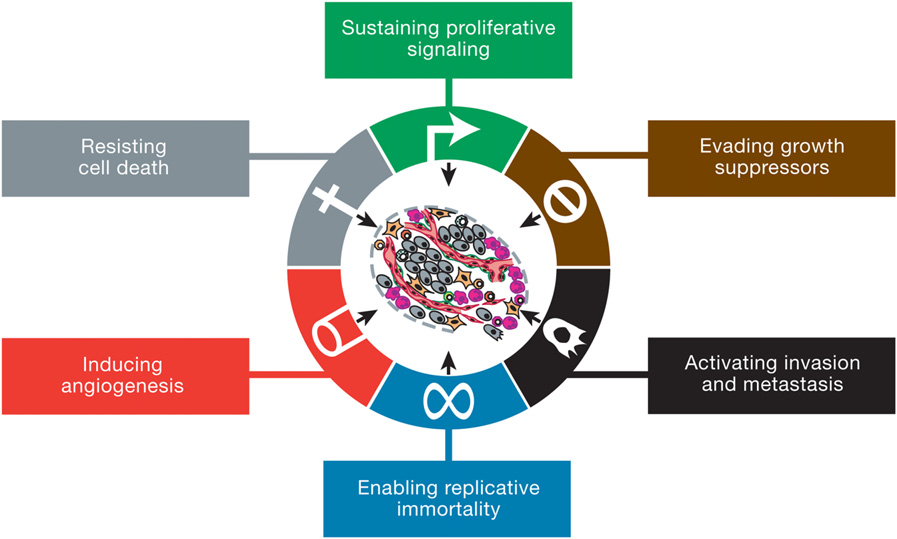
\includegraphics[width=\linewidth]{hanahan_2011_hallmarks.png}\footnotemark
\end{columns}
\footnotetext[1]{\url{https://www.cancer.gov/about-cancer/understanding/statistics}}
\footnotetext[2]{\cite{hanahan_hallmarks_2011}}
\end{frame}

\begin{frame}{Cancer is believed to be caused by somatic mutations}
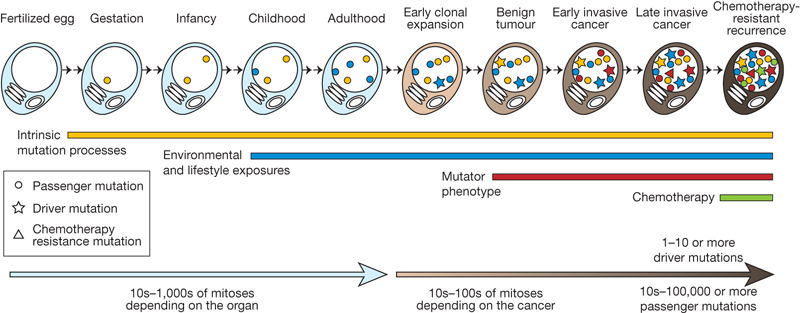
\includegraphics[width=\linewidth]{stratton_2009_mutations.jpg}
\footnotetext[1]{\cite{stratton_cancer_2009}}
\end{frame}

\begin{frame}{Understanding cancer initiation is critical for prevention}
\begin{columns}
\column{.4\textwidth}
\begin{itemize}
\item Some claim Somatic Mutation Theory doesn't explain how sufficient mutations accumulate \parencite{baker_cancer_2015}
\item Disputed evidence that lifetime cancer incidence is linearly correlated with number of somatic cell divisions \parencite{tomasetti_variation_2015}
\end{itemize}
\column{.6\textwidth}
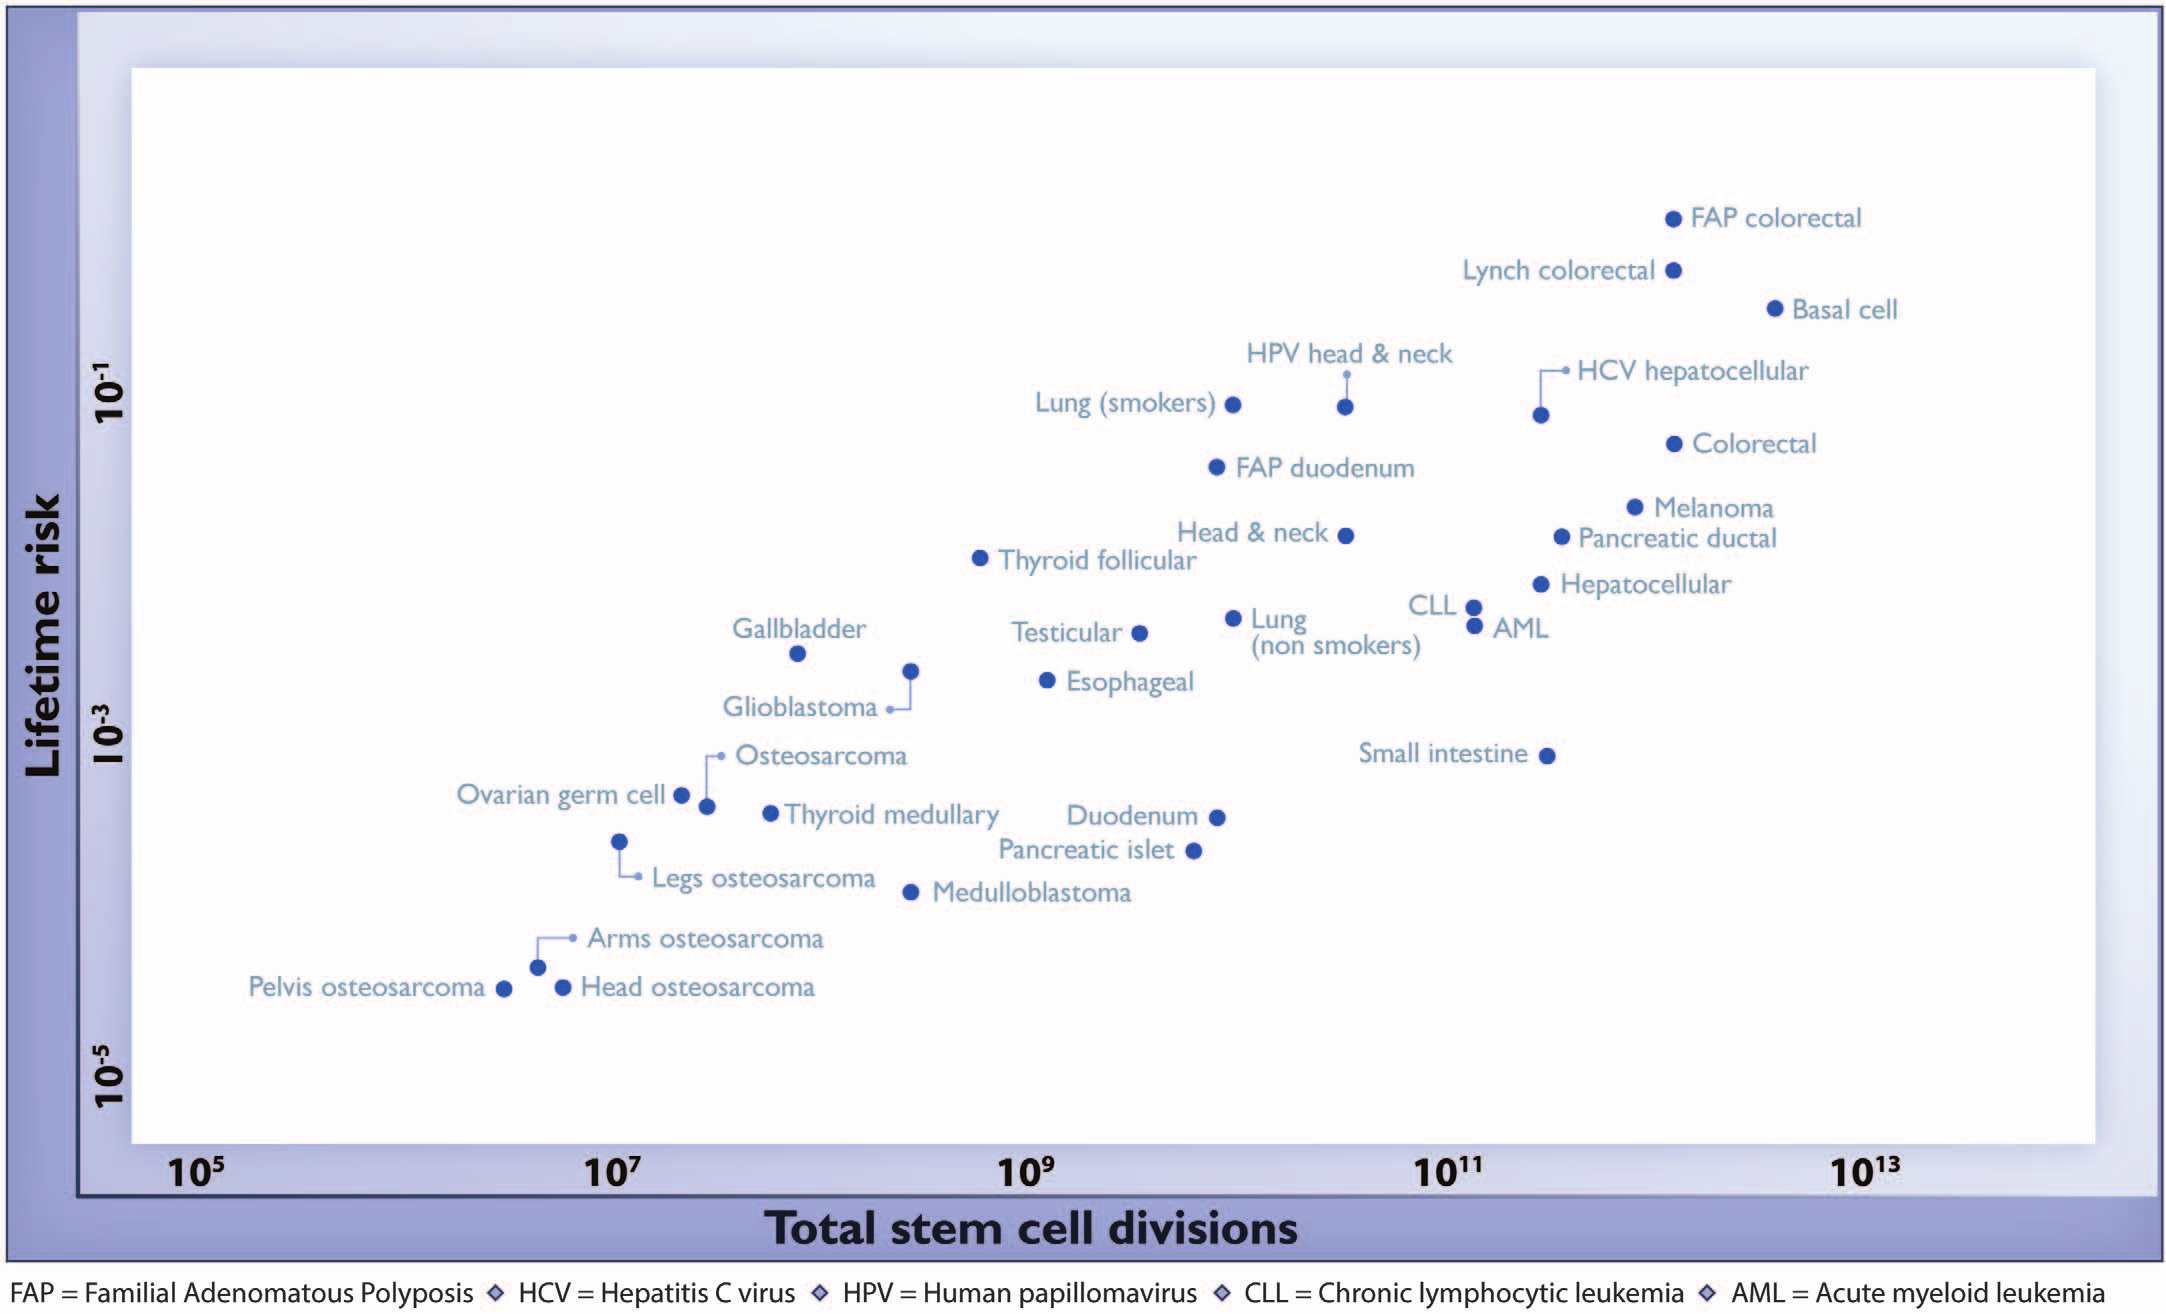
\includegraphics[width=\linewidth]{tomasetti_2015_risk.png}
\end{columns}
\footnotetext[1]{\cite{tomasetti_variation_2015}}
\end{frame}

\begin{frame}{RViMR may explain how so many mutations occur in the correct places}
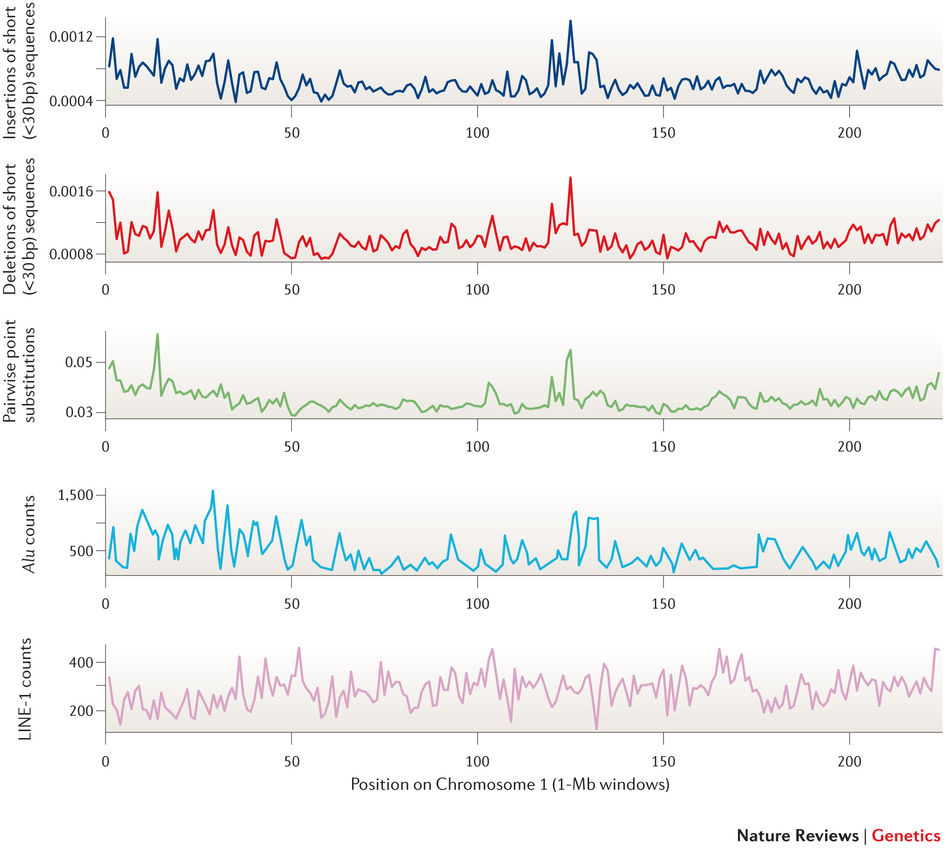
\includegraphics[width=\linewidth,trim={0 13cm 0 0},clip]{makova_2015_rvimr.jpg}
Mutation rates in 1Mb windows across chromosome 1 for different types of mutations \parencite{makova_effects_2015}
\end{frame}

\begin{frame}{Epigenetic markers significantly correlate with local mutation rate}
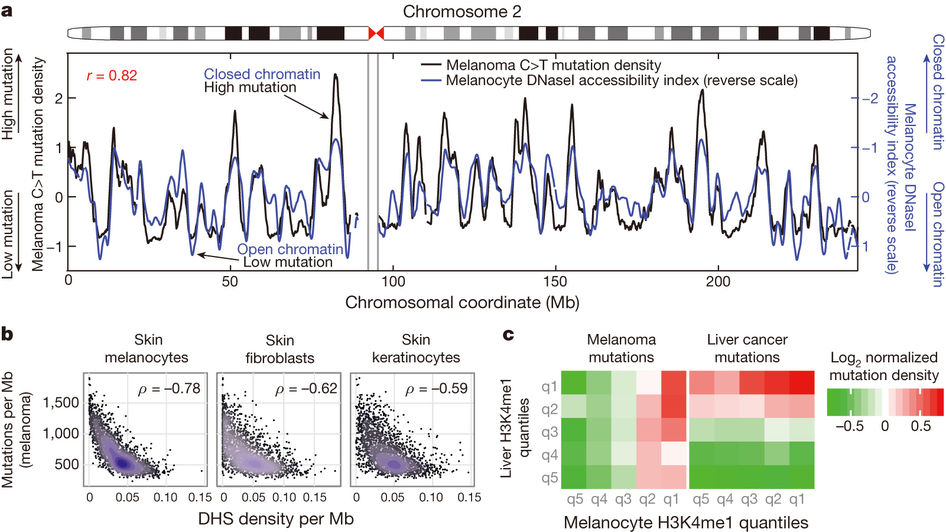
\includegraphics[width=\linewidth,trim={0 7.5cm 0 0},clip]{polak_2015_chromatin.jpg}
\begin{itemize}
\item Closed chromatin regions correlate with high single nucleotide mutation rates. 
\item Open chromatin regions correlate with high insertion/deletion rates \parencite{makova_effects_2015}
\end{itemize}
% \includegraphics[width=\linewidth]{}
\footnotetext[1]{\cite{polak_cell--origin_2015}}
\end{frame}

% \begin{frame}{Nucleosome position and occupancy affect local mutation rate}
% \begin{columns}
% \column{.4\textwidth}
% \column{.6\textwidth}
% % \includegraphics[width=\linewidth]{}
% \end{columns}
% \end{frame}

%how do we study nucleosomes?

\begin{frame}{DNAse-seq}
\begin{columns}
\column{.4\textwidth}
\column{.6\textwidth}
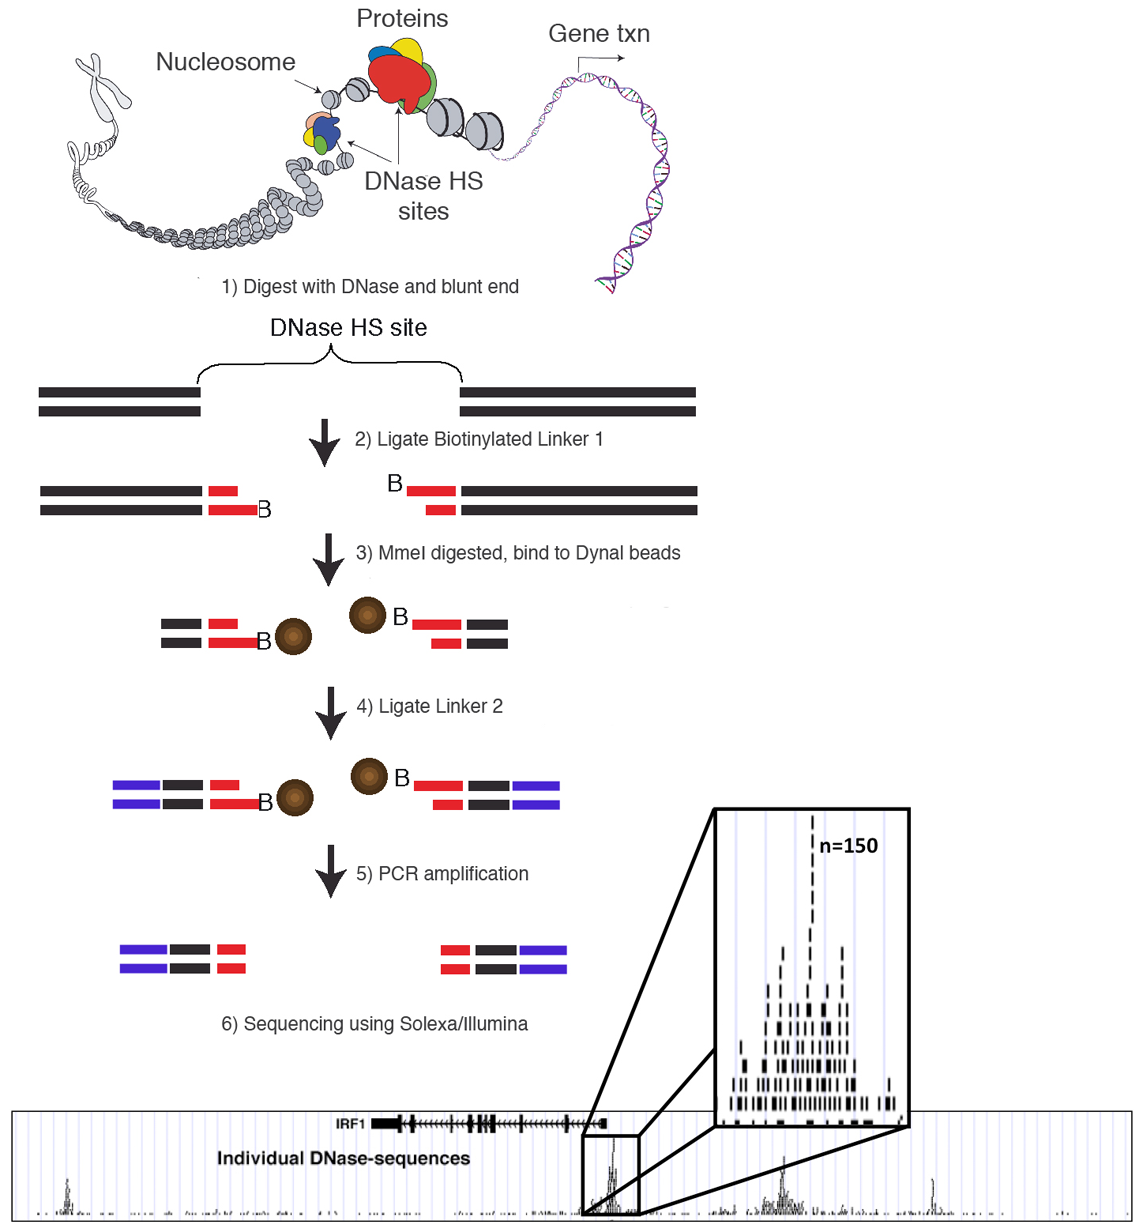
\includegraphics[width=\linewidth]{song_2010_dnase-seq.png}
\end{columns}
\footnotetext[1]{\cite{song_dnase-seq:_2010}}
\end{frame}

% \begin{frame}{ChIP-seq}
% \begin{columns}
% \column{.4\textwidth}
% \column{.6\textwidth}
% % \includegraphics[width=\linewidth]{}
% \end{columns}
% \end{frame}

\begin{frame}{Transposase}
\begin{columns}
\column{.4\textwidth}
\column{.6\textwidth}
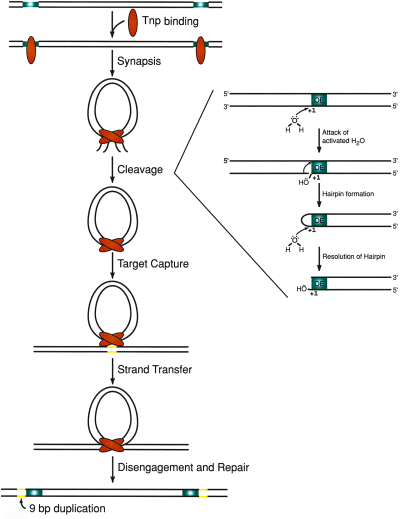
\includegraphics[width=.8\linewidth]{reznikoff_2003_tn5.png}
\end{columns}
\footnotetext[1]{\cite{reznikoff_tn5_2003}}
\end{frame}

\begin{frame}{ATAC-seq}
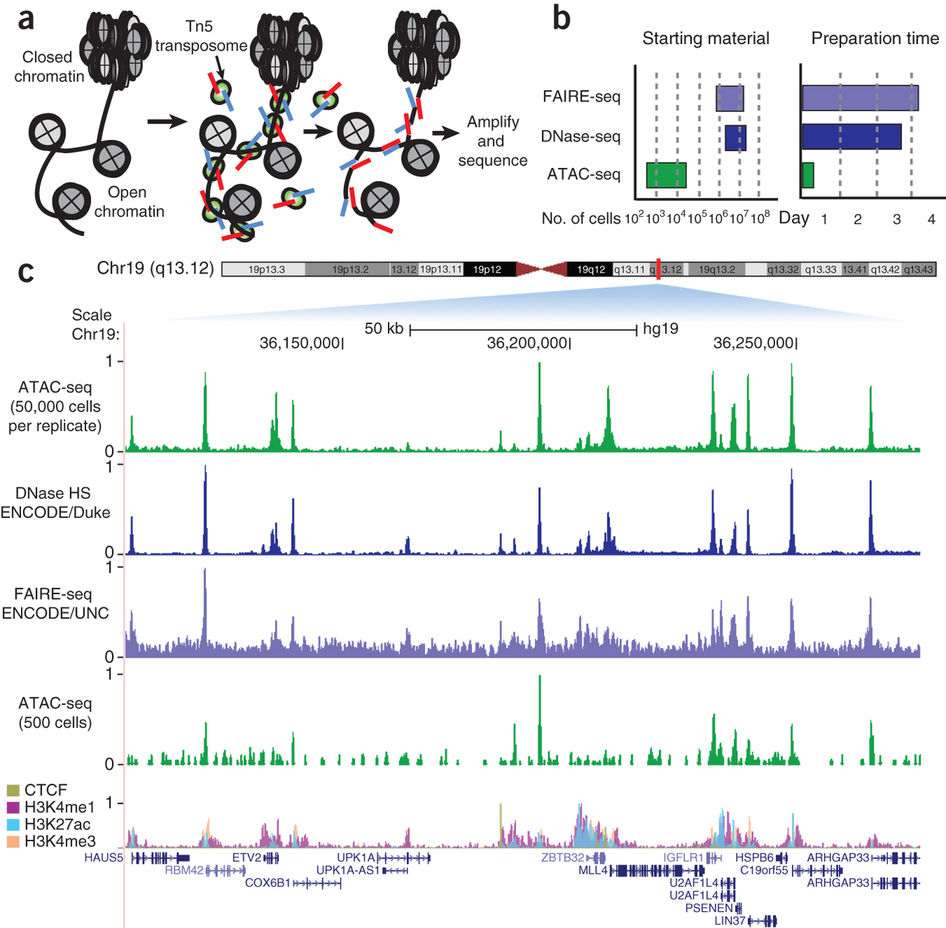
\includegraphics[width=\linewidth,trim={0 24cm 0 0},clip]{buenrostro_2013_atac.jpg}
\footnotetext[1]{\cite{buenrostro_transposition_2013}}
\end{frame}

%how do we find mutations?

\begin{frame}{Illumina Sequencing is useful for detecting SNPs}
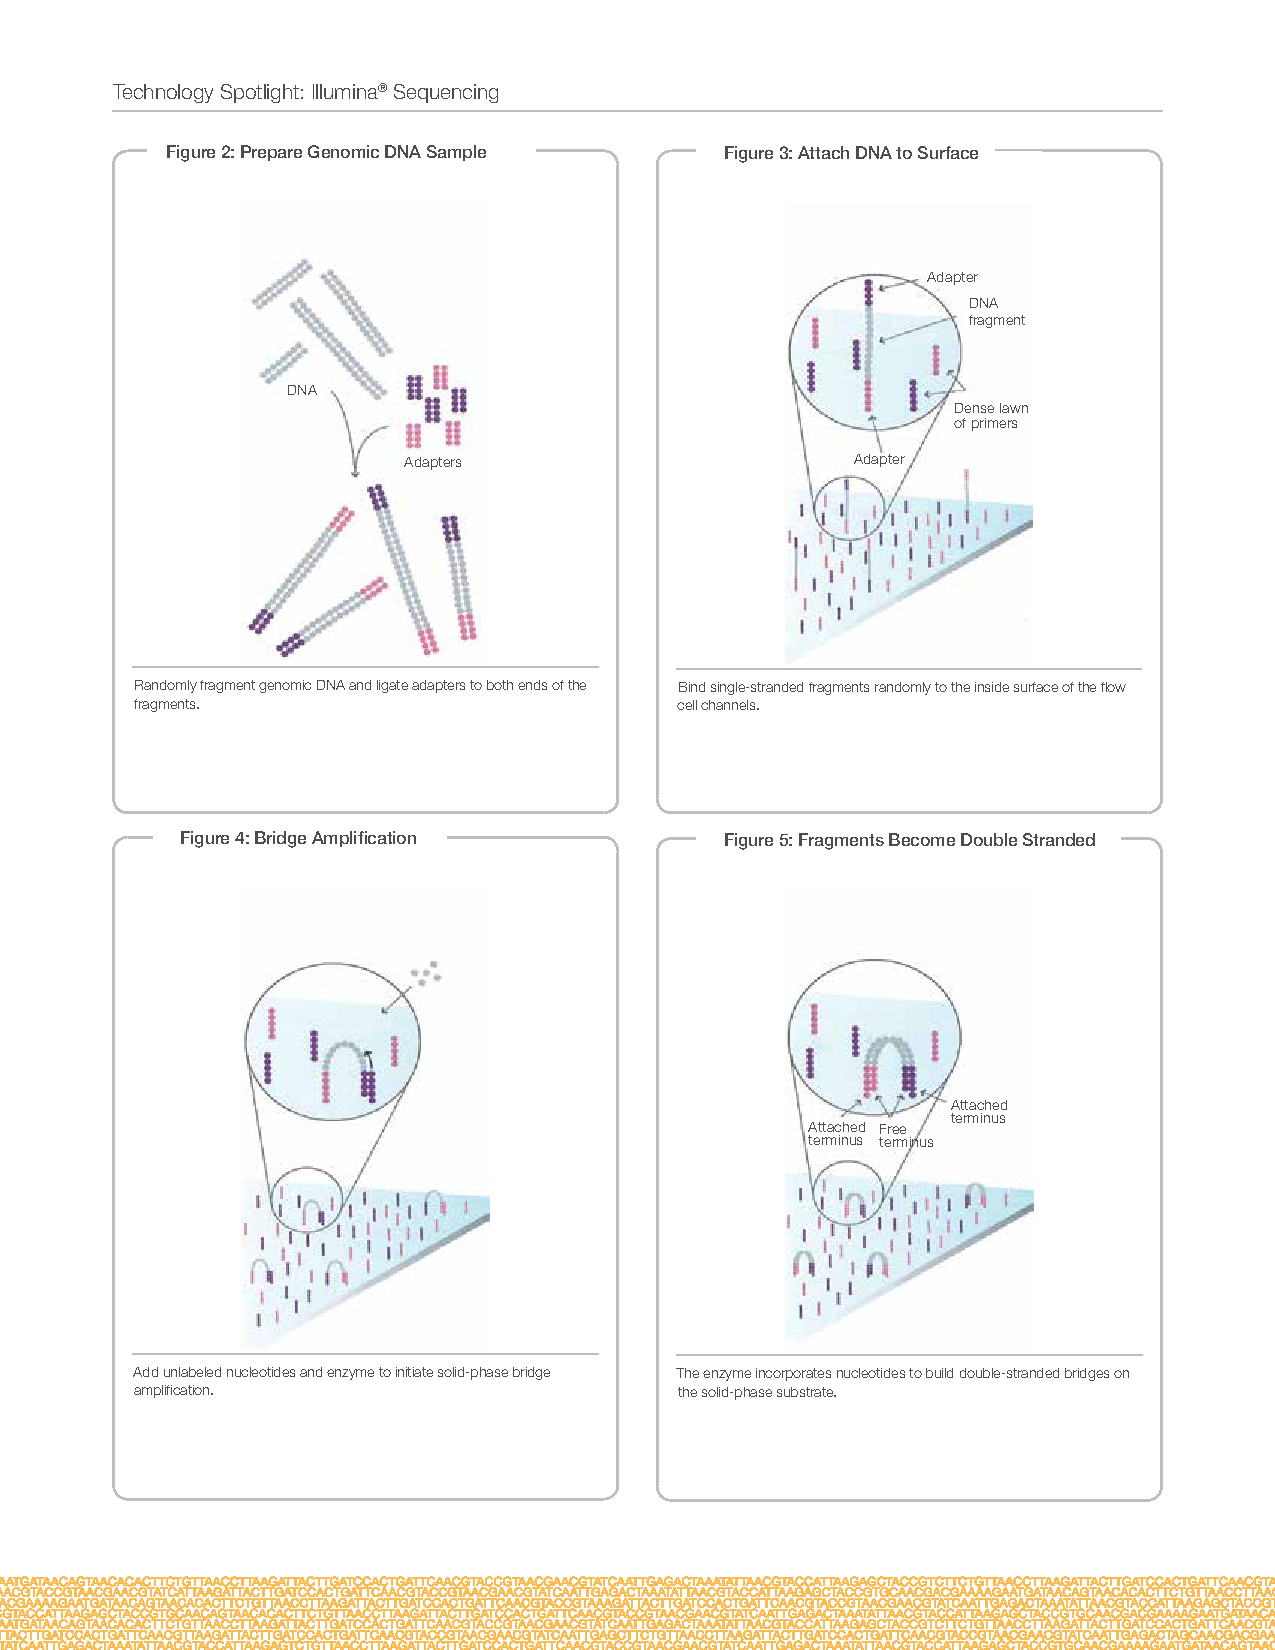
\includegraphics[width=\linewidth,trim={.5in 2.5cm .5in 14cm},clip]{illumina_techspotlight_p2.pdf}
\footnotetext[1]{\url{https://www.illumina.com/documents/products/techspotlights/techspotlight_sequencing.pdf}}
\end{frame}

\begin{frame}{Illumina Sequencing is useful for detecting SNPs}
\centering
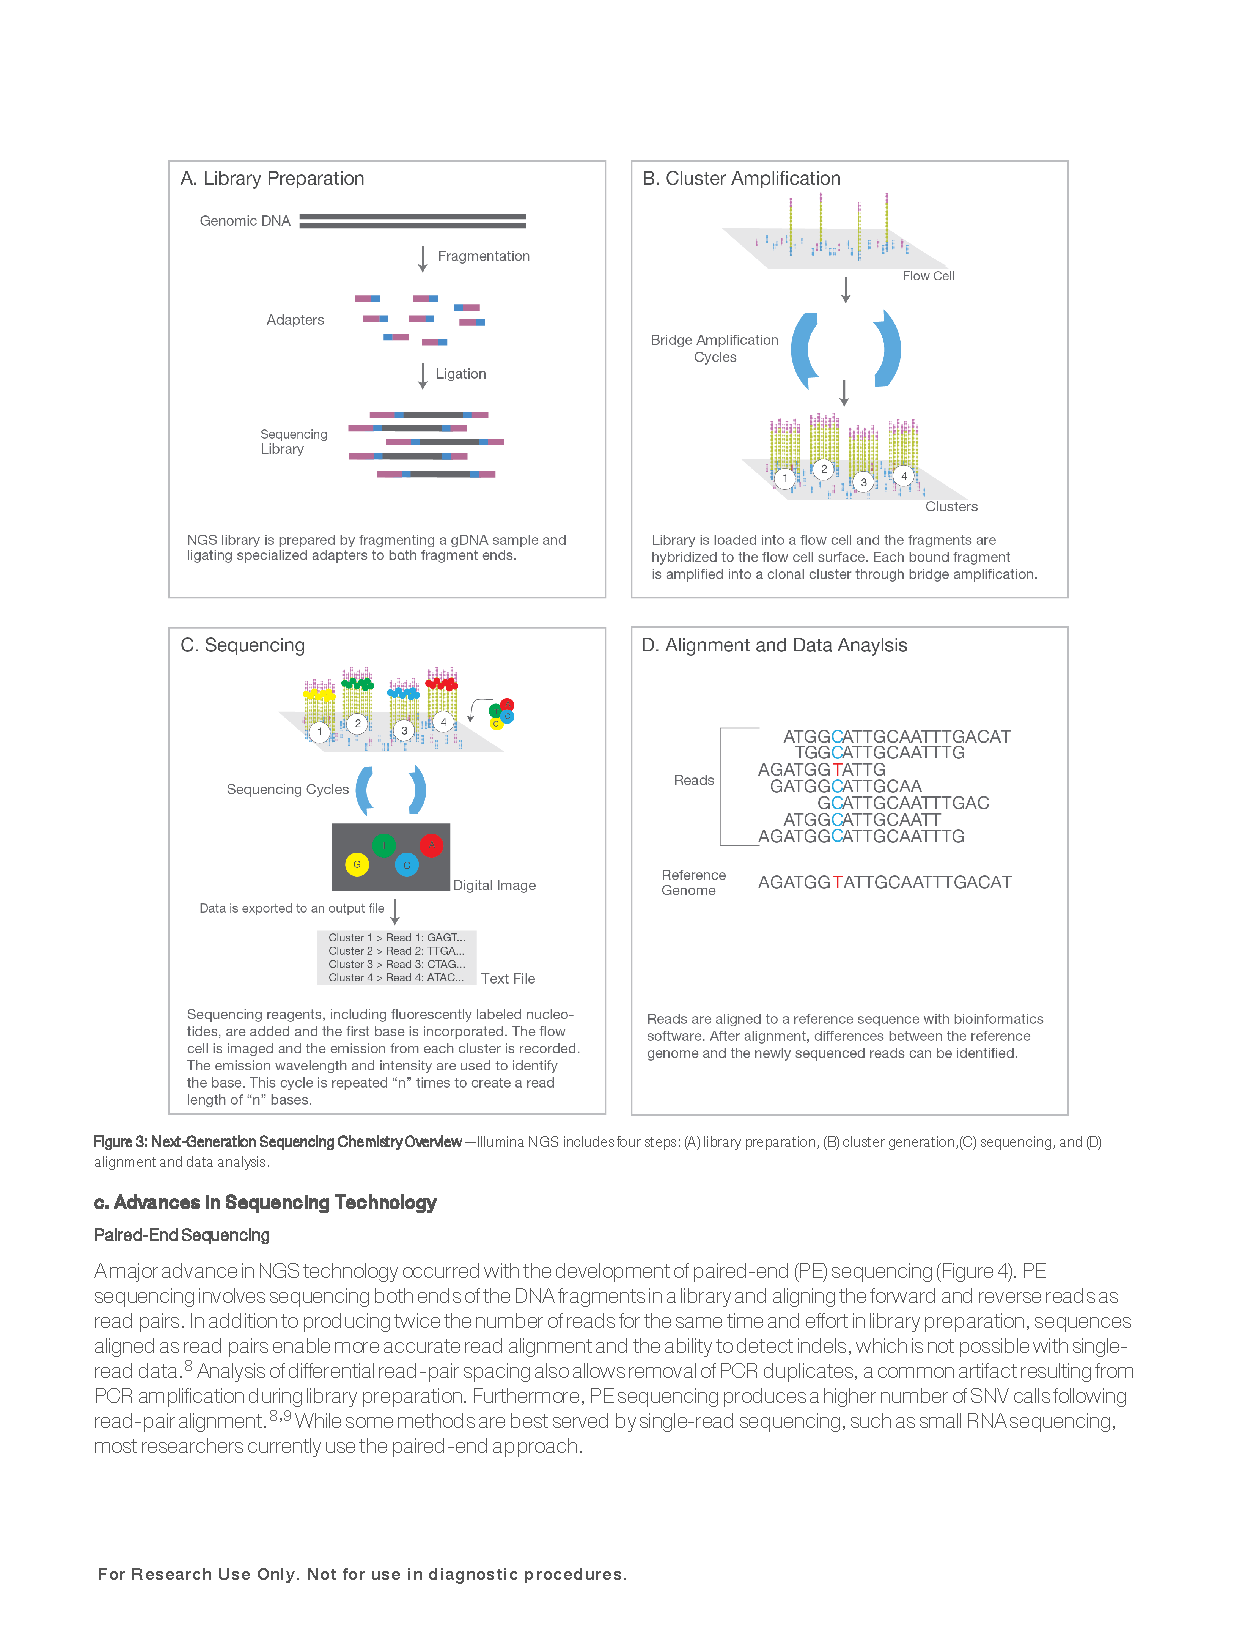
\includegraphics[width=.5\linewidth,trim={1in 9cm 4.2in 4in},clip]{illumina_intro_p5.pdf}
\footnotetext[2]{\url{https://www.illumina.com/content/dam/illumina-marketing/documents/products/illumina_sequencing_introduction.pdf}}
\end{frame}



\begin{frame}{Nanopore Sequencing is useful for detecting insertions and deletions}
\begin{columns}
\column{.4\textwidth}
\begin{itemize}
\item{A voltage is generated across the membrane containing the nanopore.}
\item{Molecules that pass through the pore cause a detectable shift in current.}
\item{$\alpha$-hemolysin is used as a biological pore}
\item{Helicase is used as a motor}
\end{itemize}
\column{.6\textwidth}
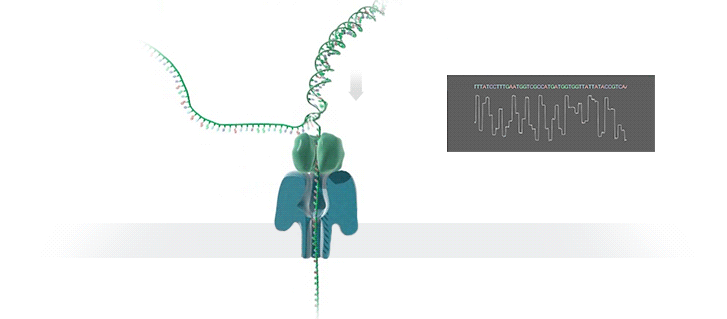
\includegraphics[width=\linewidth,trim={6cm 0 3cm 0},clip]{nanopore_seq-0.png}
\end{columns}
\footnotetext[1]{\url{https://nanoporetech.com/how-it-works}}
\end{frame}

%what do we need to consider for somatic samples?

\begin{frame}{Heterogeneity is a problem}
\begin{columns}
\column{.4\textwidth}
This can be reduced by careful sampling of tissue

\column{.6\textwidth}
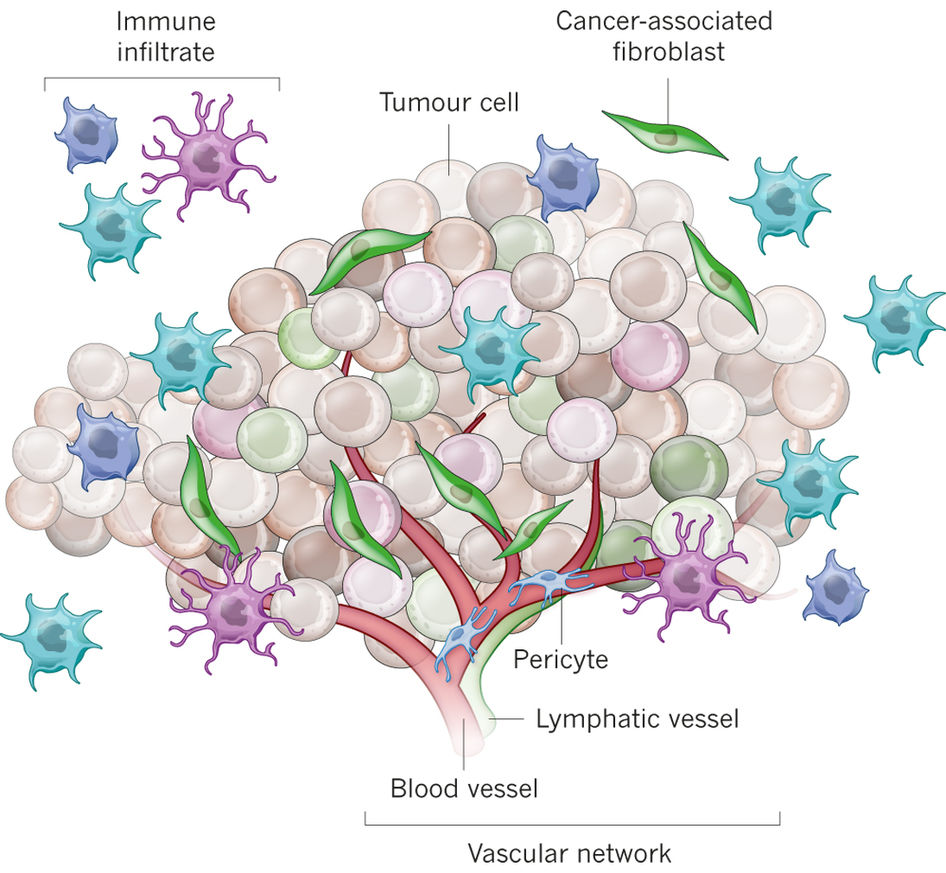
\includegraphics[width=\linewidth]{junttila_2013_heterogeneity.jpg}
\end{columns}
\footnotetext[1]{\cite{junttila_influence_2013}}
\end{frame}

\begin{frame}{Sequencing errors are a problem}
These errors are caused by
\begin{itemize}
\item DNA damage
\item Mutations during library preparation
\item Sequencer measurement error
\end{itemize}

The first two can be minimized by careful DNA extraction methods and minimizing the number of PCR steps required before sequencing.

\vskip 1em

Remaining errors can be corrected \textit{in silico}
\end{frame}

\begin{frame}{Read correction reduces errors}
\begin{columns}
\column{.5\textwidth}
In short reads:
\begin{enumerate}
	\item Create K-mer frequency table
	\item For every read containing a unique K-mer, change the base to one that will make the K-mer non unique
\end{enumerate}
\column{.5\textwidth}
In long reads:
\begin{itemize}
	\item The reads are long enough that there is a significant level of overlap between reads. Use this overlap to find a consensus.
	\item \textbf{Or} align short reads to the long reads to "polish" the long reads and repair errors.
\end{itemize}
\end{columns}
\end{frame}

%with all this in mind, our aims!

\begin{frame}{Aims}
How does chromatin accessibility correlate with mutation rate in the same tissue? How does it change in cancer?

\vskip 1em

\textbf{Aim 1}: Develop a bioinformatic pipeline to detect somatic mutations and estimate chromatin accessibility across the genome in somatic samples.
\begin{itemize}
	\item Use long reads for structural variation, short reads for single nucleotide changes
	\item Error correct reads
\end{itemize}

\vskip 1em

\textbf{Aim 2}: Test the hypothesis that chromatin accessibility significantly impacts mutation rate.
\begin{itemize}
	\item Poisson test
	\item Non-parametric test of ATAC-seq enrichment at mutated sites
	\item Logistic regression of ATAC-seq enrichment
\end{itemize}
\end{frame}

%pipeline stuff
%for the pipeline, do left half text, right half highlight the part of the pipeline we're talking about

\begin{frame}{Pipeline Overview}
\centering
\includegraphics[width=.7\linewidth]{figure.pdf}
\end{frame}

\begin{frame}{Pipeline Validation}
\begin{columns}
\column{.4\textwidth}
\column{.6\textwidth}
% \includegraphics[width=\linewidth]{}
\end{columns}
\end{frame}

\begin{frame}{Short Read Correction - Rcorrector}
\begin{columns}
\column{.4\textwidth}
\column{.6\textwidth}
% \includegraphics[width=\linewidth]{}
\end{columns}
\end{frame}

\begin{frame}{Long Read Correction - Nanocorr}
\begin{columns}
\column{.4\textwidth}
\column{.6\textwidth}
% \includegraphics[width=\linewidth]{}
\end{columns}
\end{frame}

\begin{frame}{Alignment - Minimap2}
\begin{columns}
\column{.4\textwidth}
\column{.6\textwidth}
% \includegraphics[width=\linewidth]{}
\end{columns}
\end{frame}

\begin{frame}{Detect Mutations - MuTect2}
\begin{columns}
\column{.4\textwidth}
\column{.6\textwidth}
% \includegraphics[width=\linewidth]{}
\end{columns}
\end{frame}

\begin{frame}{Detect Mutations - Nanopolish}
\begin{columns}
\column{.4\textwidth}
\column{.6\textwidth}
% \includegraphics[width=\linewidth]{}
\end{columns}
\end{frame}

\begin{frame}{Calculate Chromatin Accessibility - MACS2}
\begin{columns}
\column{.4\textwidth}
\column{.6\textwidth}
% \includegraphics[width=\linewidth]{}
\end{columns}
\end{frame}

\begin{frame}{Tissue Collection}
\begin{columns}
\column{.5\linewidth}
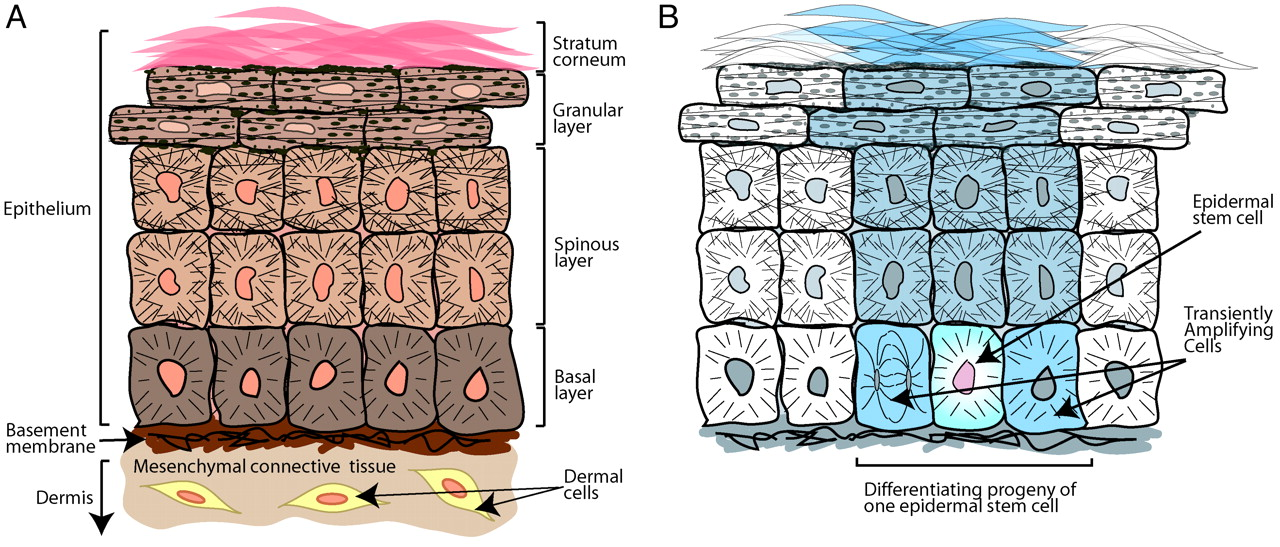
\includegraphics[width=\linewidth]{alonso_2003_skin.jpg}
\column{.5\linewidth}
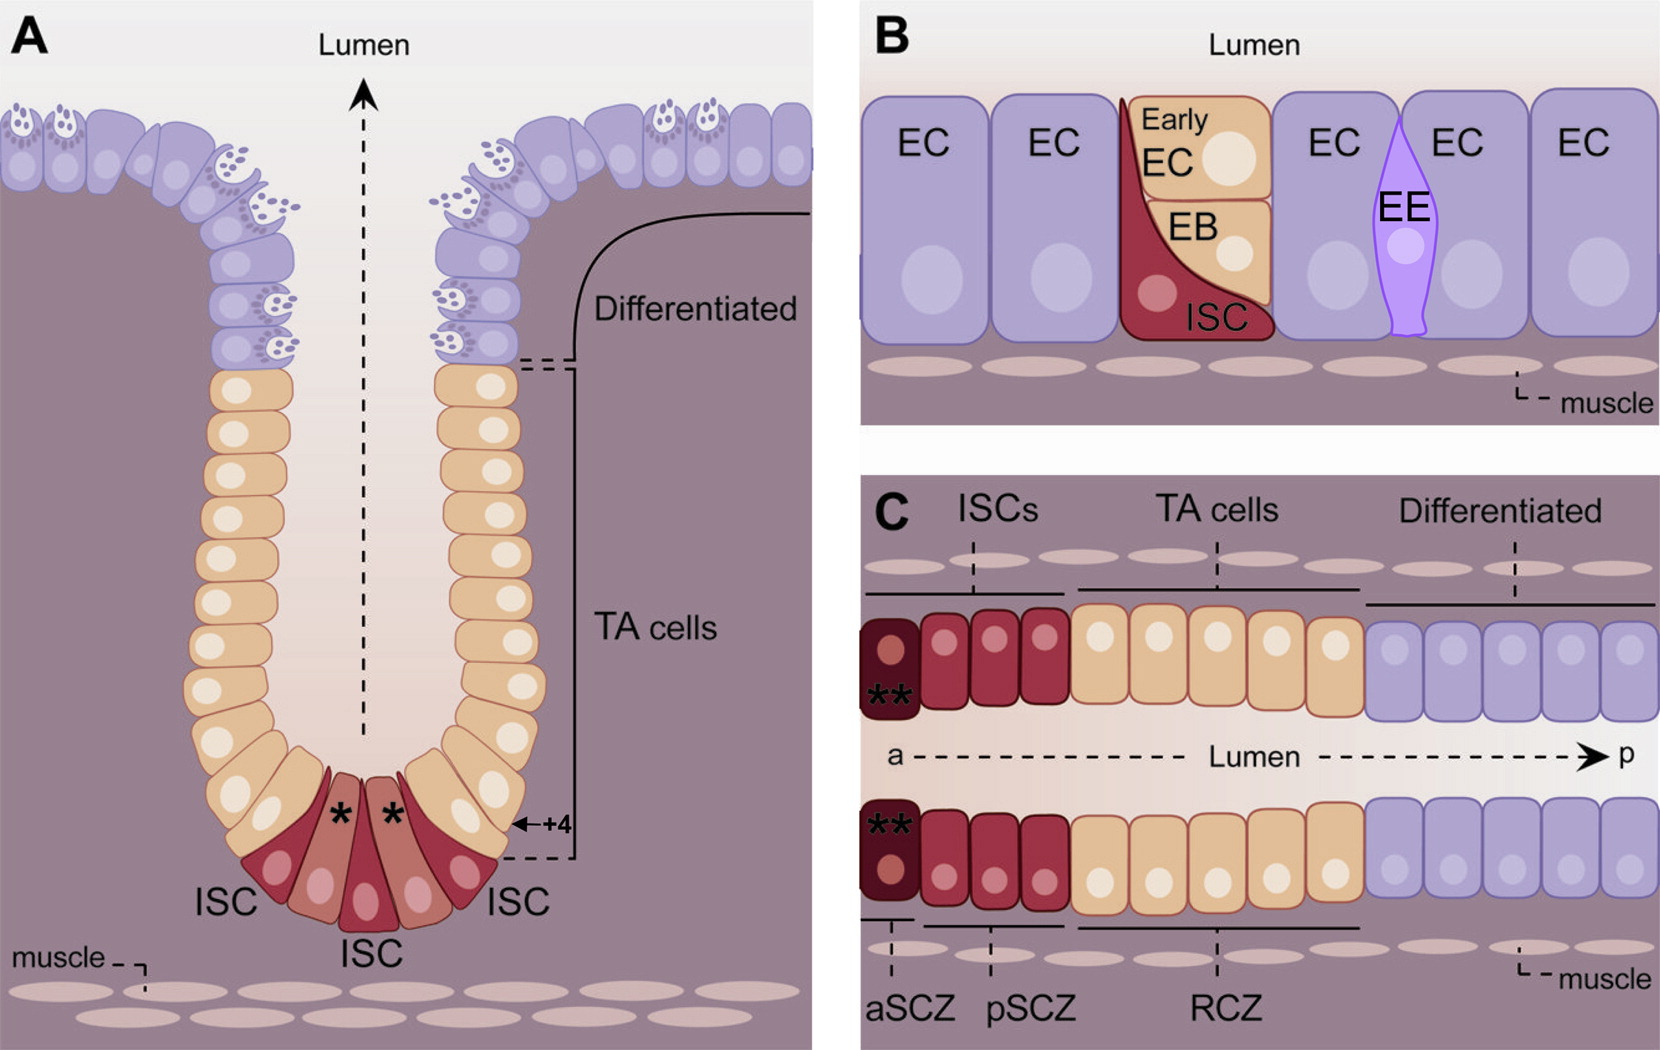
\includegraphics[width=\linewidth]{casali_2009_intestine.jpg}
\end{columns}
\footnotetext[1]{\cite{alonso_stem_2003}}
\footnotetext[2]{\cite{casali_intestinal_2009}}
\end{frame}

\begin{frame}{Library Construction}
\end{frame}

\begin{frame}{Statistical Analysis}
\end{frame}

\begin{frame}{Expected Results - Mutation Rates in Open and Closed Chromatin}
\end{frame}

\begin{frame}{Expected Results - Distribution of Chromatin State at Mutated Sites}
\end{frame}

\begin{frame}{Expected Results - Logistic Regression}
\end{frame}

\begin{frame}{Conclusion}
\end{frame}

\begin{frame}[t, allowframebreaks]
\frametitle{References}
\printbibliography
\end{frame}

\end{document}